\section{Crowd Counting}
\subsection{Implementation Details}
\subsubsection{Dataset}
The ShanghaiTech dataset \cite{zhang2016single} is divided into two parts: Part A and Part B. Each part contains two subfolders: train\_data and test\_data, corresponding to the training and testing sets. Within each of these folders, there are two additional subfolders: images and ground\_truth. The images folder contains .jpg images, while the ground\_truth folder contains .mat files (in MATLAB format), where each file stores head annotation coordinates corresponding to each image. Additionally, the image resolutions differ between the two parts: Part A includes high-resolution images with very high crowd density, whereas Part B contains surveillance camera images with lower crowd density and a fixed resolution of 768 × 1024.\\

\begin{figure}[H]
    \centering 
    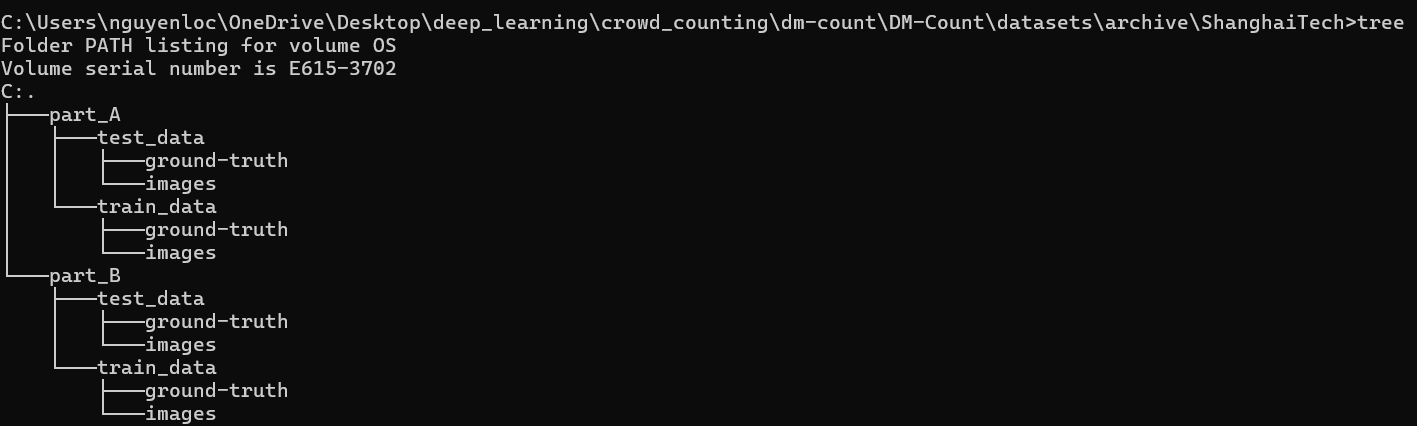
\includegraphics[width=15cm]{experiment/images/tree.png} 
    \caption{The structure of ShanghaiTech} 
    \label{fig:sh_structure}
\end{figure}

In this project, the focus is primarily on Part B of the dataset, as it better represents real-world surveillance scenarios with moderate crowd levels and consistent image quality.

\begin{figure}[H]
    \centering
    \begin{subfigure}{0.4\textwidth} 
        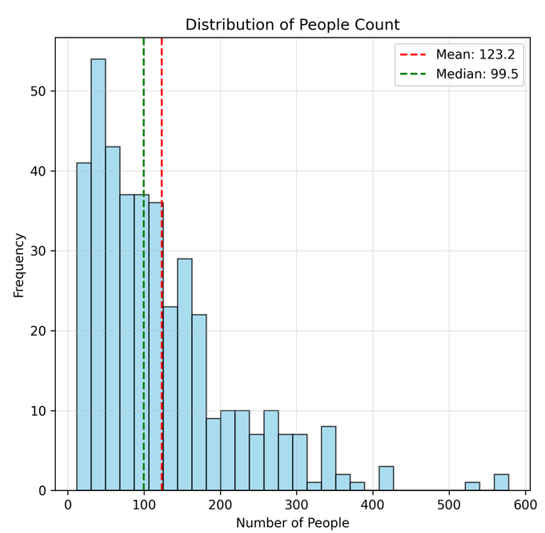
\includegraphics[width=\linewidth]{experiment/images/distrubution.png}
        \caption{Distribution of People Count}
        \label{fig:dist}
    \end{subfigure}
    \hspace{1mm}
    \begin{subfigure}{0.425\textwidth}
        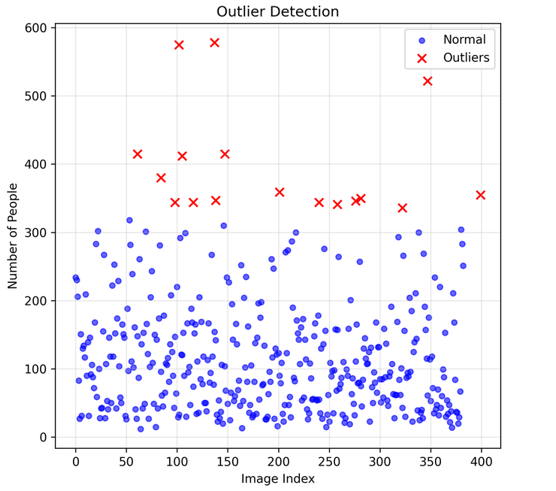
\includegraphics[width=\linewidth]{experiment/images/outlier.png}
        \caption{Outlier Detection}
        \label{fig:outlier}
    \end{subfigure}
    \hspace{1mm}
    \begin{subfigure}{0.4\textwidth}
        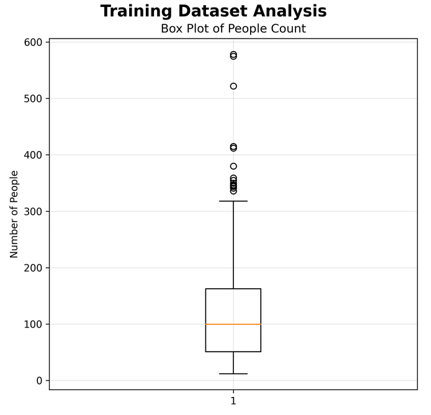
\includegraphics[width=\linewidth]{experiment/images/boxplot.png}
        \caption{Boxplot of People Count}
        \label{fig:boxplot}
    \end{subfigure}
        \begin{subfigure}{0.435\textwidth}
        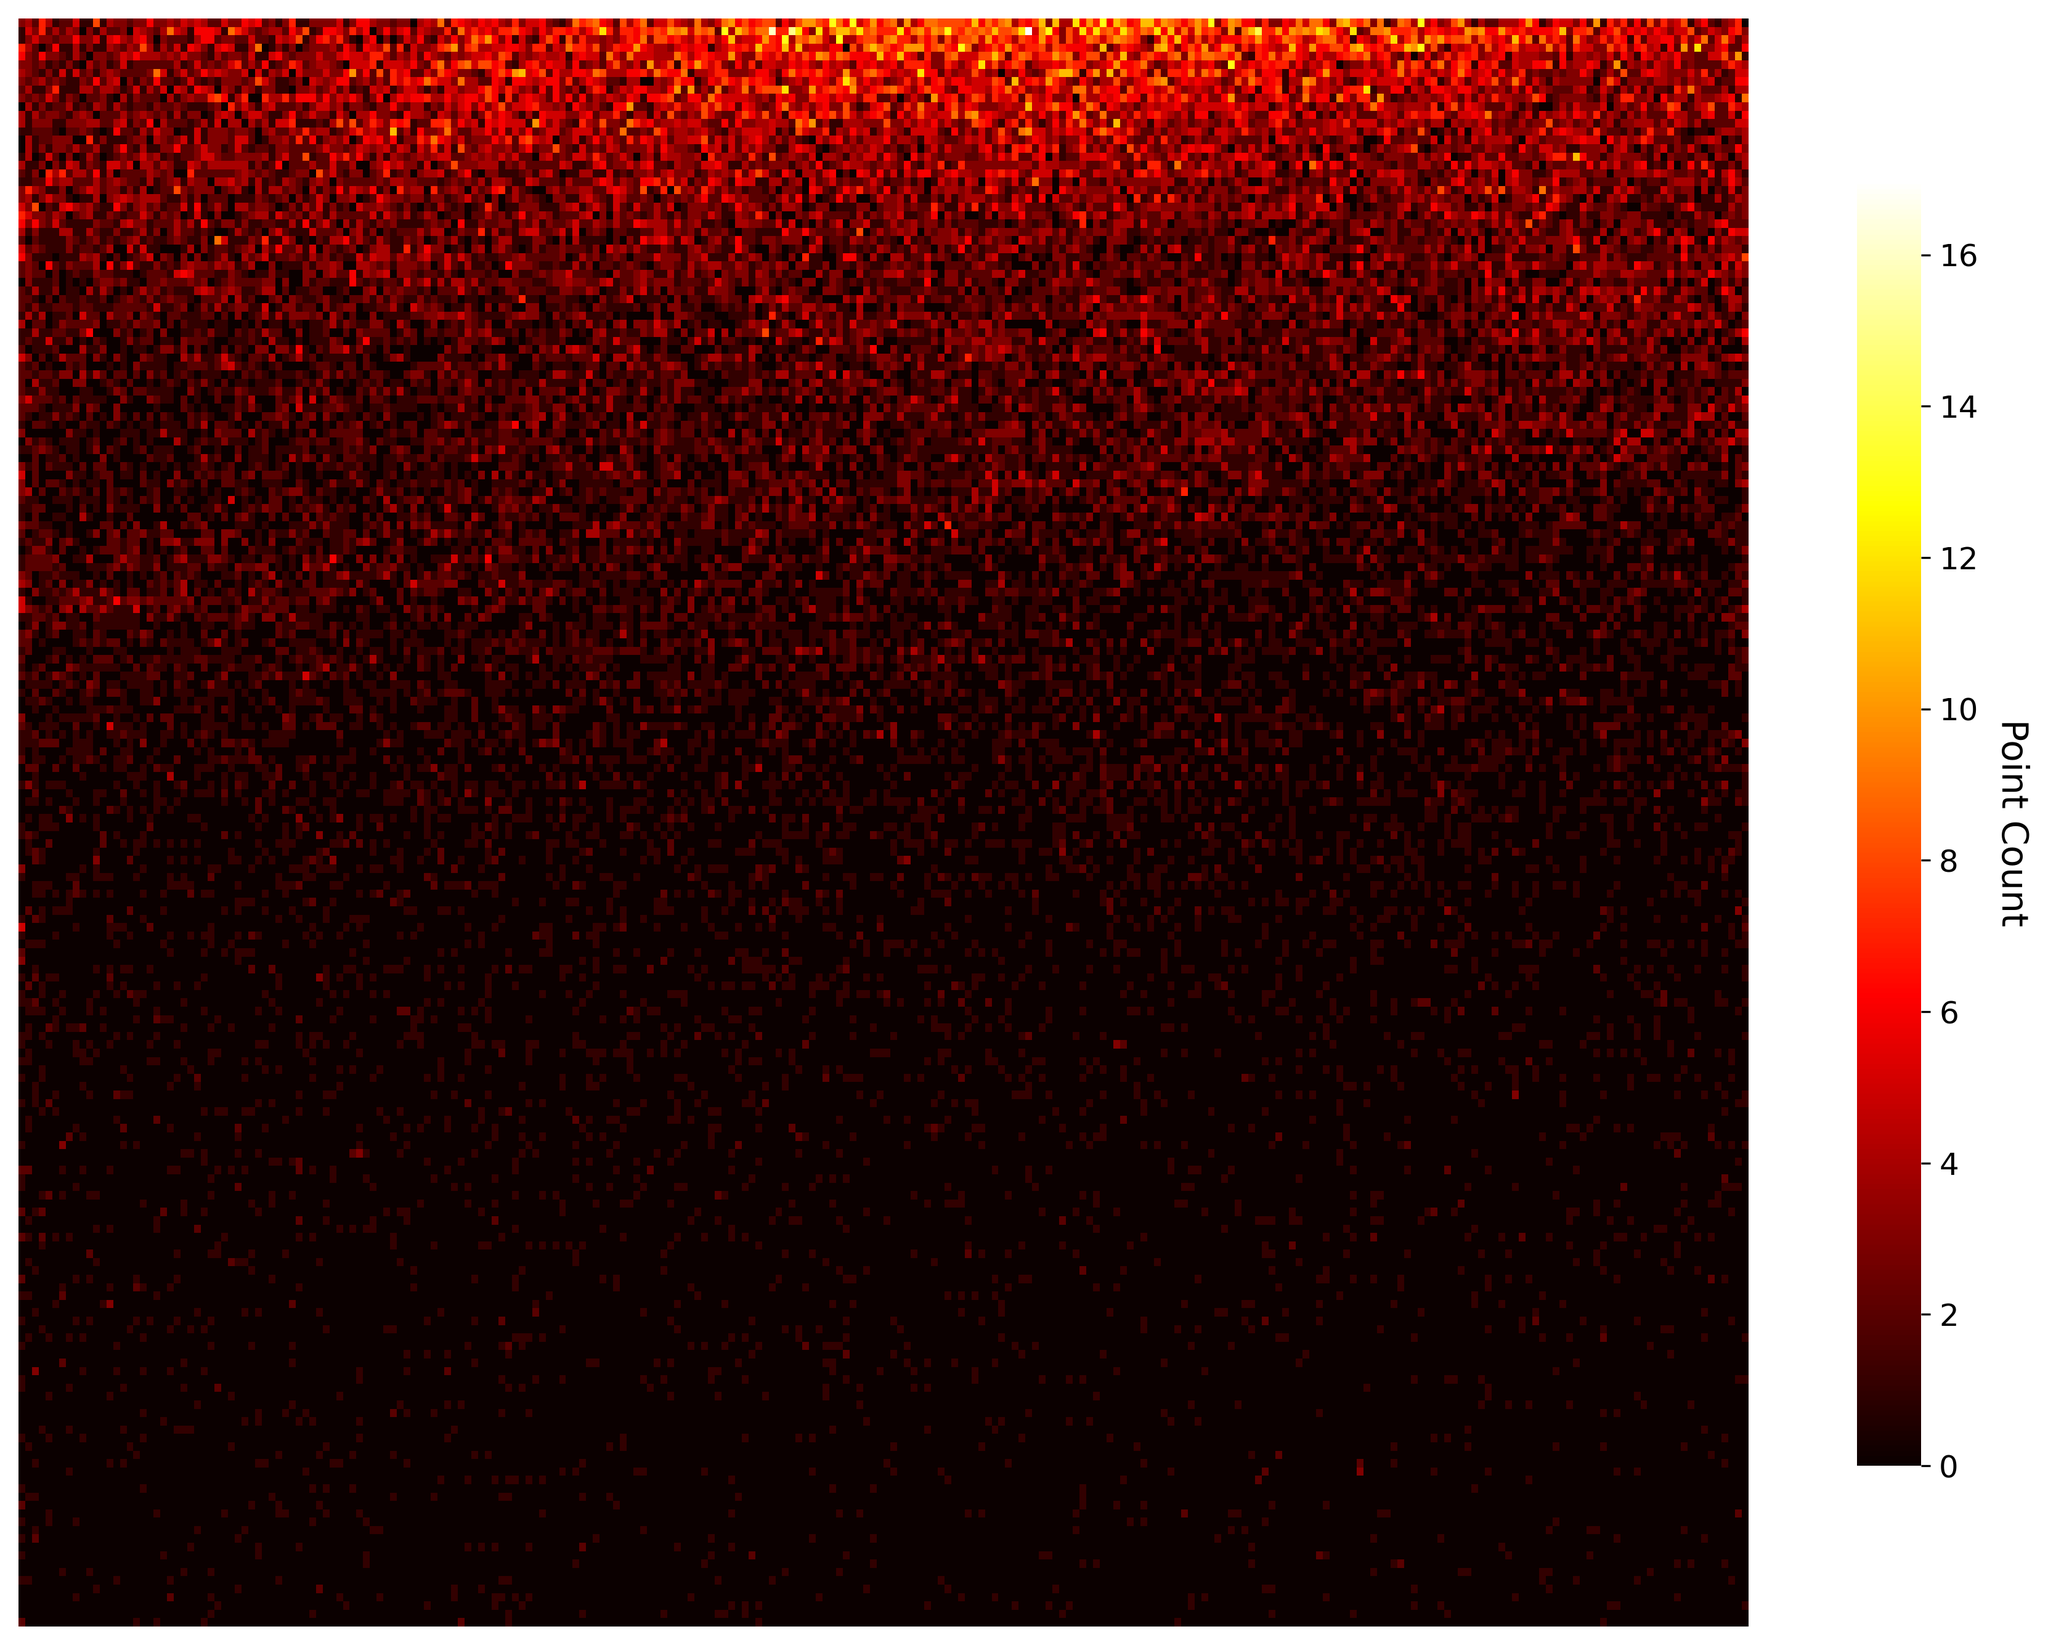
\includegraphics[width=\linewidth]{experiment/images/red.png}
        \caption{Absolute Point Density}
        \label{fig:heatmap}
    \end{subfigure}
    \caption{Overview of SHB\_Train}
    \label{fig:shb_samples}
\end{figure}
Figure~\ref{fig:shb_samples} presents a statistical overview of the SHB\_Train dataset. Subfigure~\ref{fig:dist} shows that most images contain fewer than 200 people, with a heavily right-skewed distribution due to a few highly crowded scenes. The average count is 123.2, and the median is 99.5, indicating a concentration in low to medium-density levels. Subfigure~\ref{fig:outlier} highlights outliers — images with more than 300 people — which could affect model stability during training. \\
The boxplot in subfigure~\ref{fig:boxplot} confirms this skewed distribution and emphasizes the presence of multiple outliers. Subfigure~\ref{fig:heatmap} provides a heatmap of head annotation density aggregated across all training images. Warmer colors (yellow to white) indicate areas with higher concentration of head annotations. It is evident that annotations are predominantly clustered in the upper region of the image, while the lower part remains sparsely populated. This spatial imbalance could introduce bias during training. To mitigate this, techniques such as spatial-aware data augmentation, random cropping, or attention-based modules may help improve model generalization in real-world settings.\\
Figure~\ref{fig:examples_imgs}, Figure~\ref{fig:examples_annot} present four representative examples from the SHB\_Train dataset, including both the original images and their corresponding annotations. The selected images cover a range of crowd densities, from sparse scenes with only a few individuals to more populated areas. These scenes maintain a consistent resolution of 768 × 1024 and were captured from similar camera angles, making the dataset well-suited for surveillance-based crowd analysis. The diversity in lighting conditions, backgrounds, and degrees of occlusion further contributes to the robustness of models trained on this data. In the annotation images, each dot indicates the location of a person’s head, based on the ground-truth points provided in the dataset’s .mat files. These annotations offer precise localization even in challenging conditions and serve as the foundation for generating density maps in supervised learning.
\begin{figure}[H]
    \centering
    \begin{subfigure}{0.23\textwidth}
        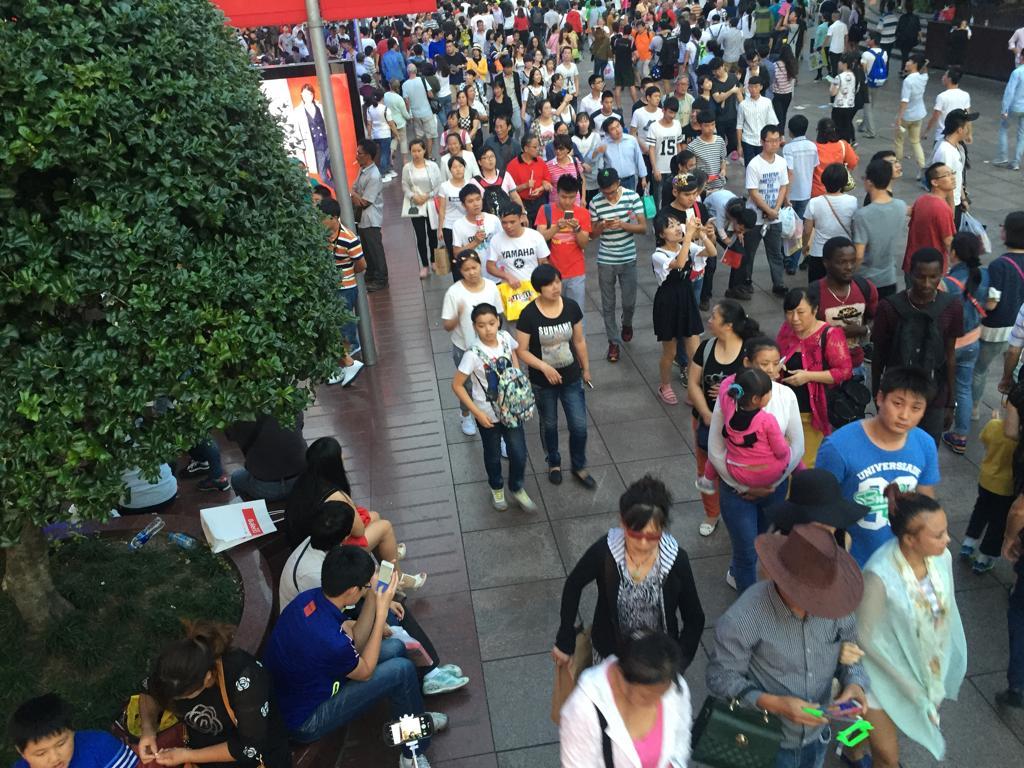
\includegraphics[width=\linewidth]{experiment/images/IMG_1.jpg}
    \end{subfigure}
    \hfill
    \begin{subfigure}{0.23\textwidth}
        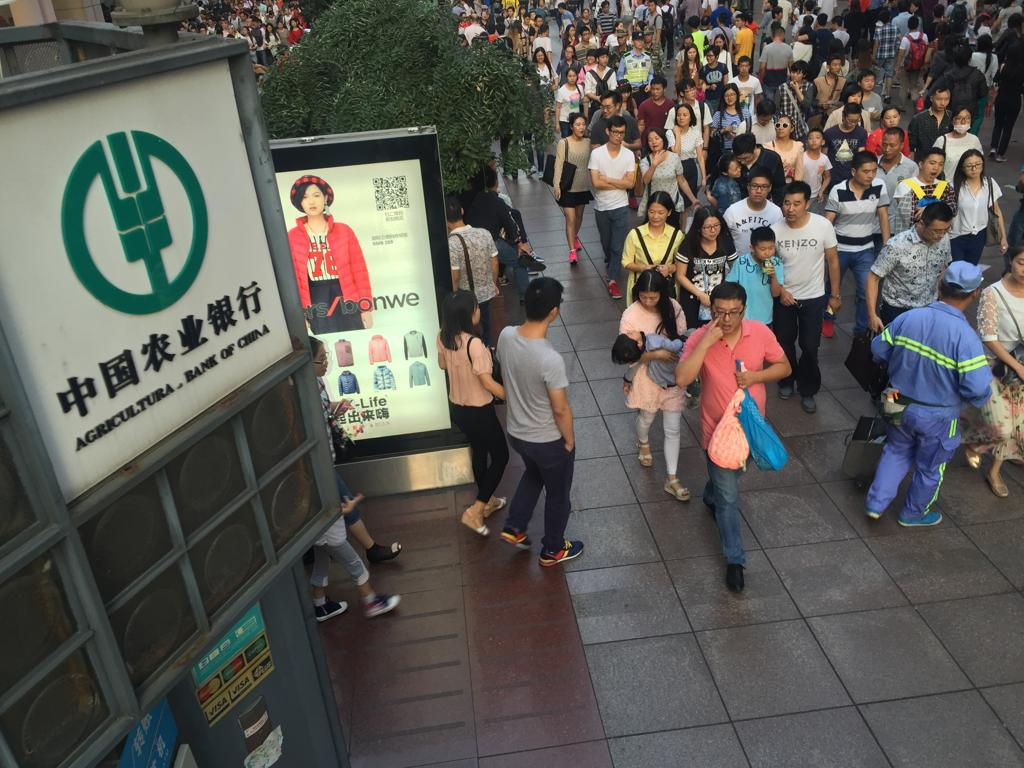
\includegraphics[width=\linewidth]{experiment/images/IMG_2.jpg}
    \end{subfigure}
    \hfill
    \begin{subfigure}{0.23\textwidth}
        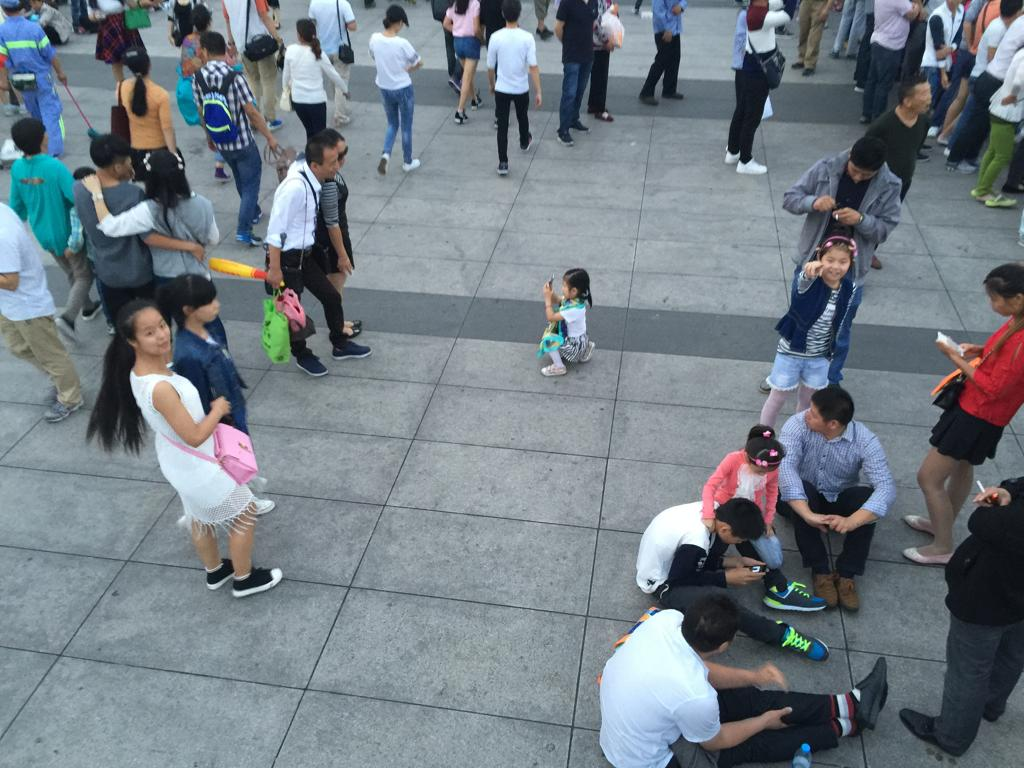
\includegraphics[width=\linewidth]{experiment/images/IMG_3.jpg}
    \end{subfigure}
    \hfill
    \begin{subfigure}{0.23\textwidth}
        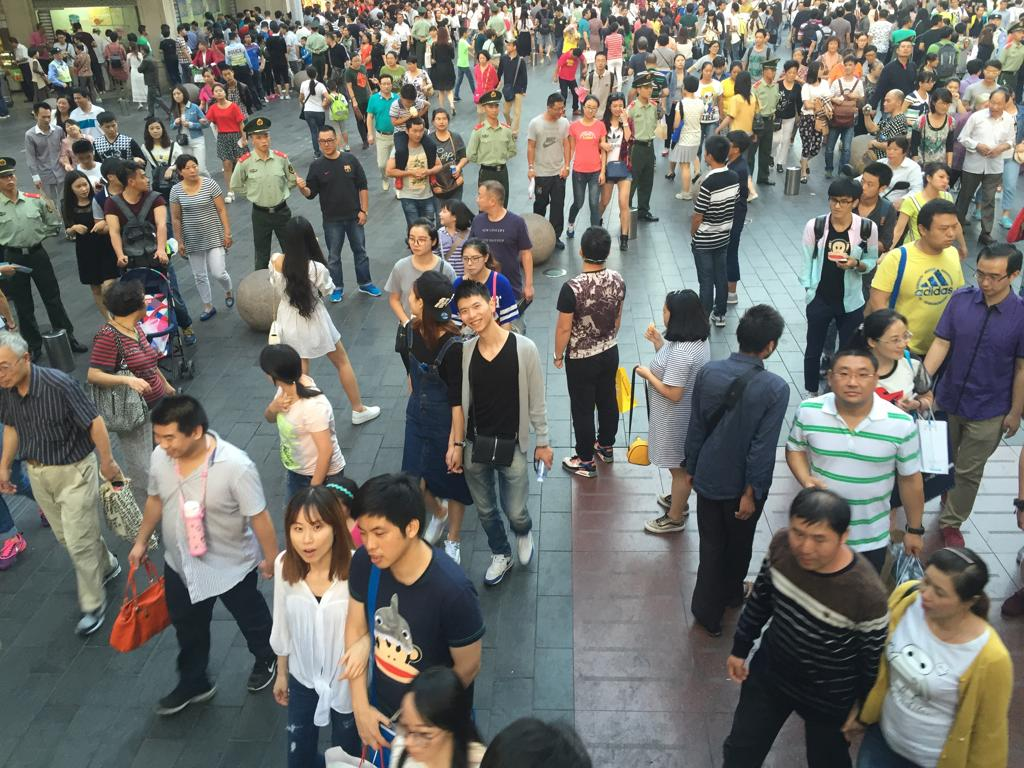
\includegraphics[width=\linewidth]{experiment/images/IMG_4.jpg}
    \end{subfigure}
    \caption{Images from SHB\_Train dataset}
    \label{fig:examples_imgs}
\end{figure}
\begin{figure}[H]
    \centering 
    \begin{subfigure}{0.23\textwidth}
        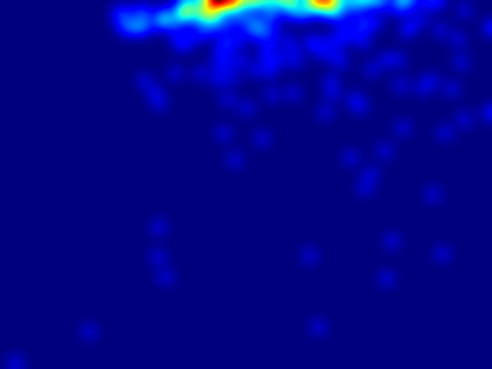
\includegraphics[width=\linewidth]{experiment/images/IMG_1_mat.png}
    \end{subfigure}
    \hfill
    \begin{subfigure}{0.23\textwidth}
        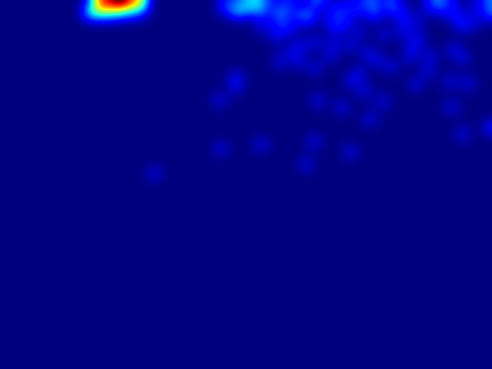
\includegraphics[width=\linewidth]{experiment/images/IMG_2_mat.png}
    \end{subfigure}
    \hfill
    \begin{subfigure}{0.23\textwidth}
        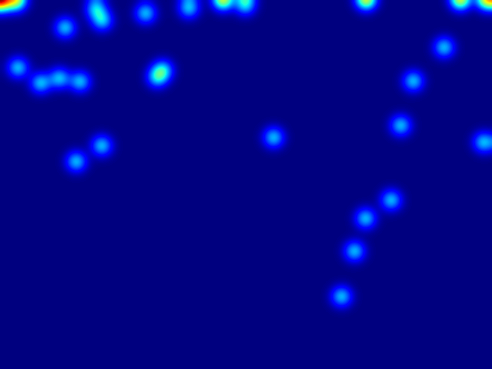
\includegraphics[width=\linewidth]{experiment/images/IMG_3_mat.png}
    \end{subfigure}
    \hfill
    \begin{subfigure}{0.23\textwidth}
        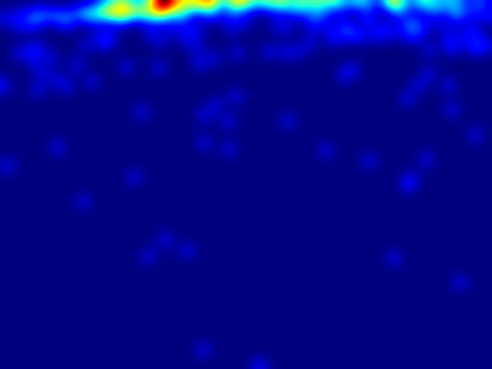
\includegraphics[width=\linewidth]{experiment/images/IMG_4_mat.png}
    \end{subfigure}
    \caption{Annonations from SHB\_Train dataset}
    \label{fig:examples_annot}
\end{figure}
\subsubsection{Training Settings and Hyperparameters}
\textbf{FFNet: } The backbone of FFNet is the official ConvNeXt-Tiny model, which is pretrained on the ImageNet-1k dataset. In our experiments, data augmentation was limited to random cropping and random horizontal flipping. For SHB, we set the cropping size to 512  The model training utilized the AdamW optimizer with a batch size of 8, and the initial learning rate was set to 1e-5. Additionally, to mitigate overfitting, we introduced an L2 regularization term with a coefficient of 0.005. All experiments were conducted using PyTorch on a single 16-GB RTX 4080. \\
\textbf{Yolov11: }Environment
        \begin{itemize}
            \item GPU: 1× NVIDIA RTX 2080 (8 GB VRAM)
            \item Epochs: 500
            \item Crop size: 512
            \item Batch size: 16
            \item Learning rate: 1e-5
        \end{itemize}
\textbf{CCTrans: }Environment
        \begin{itemize}
            \item GPU: 1× NVIDIA RTX 4060 Ti (16 GB VRAM)
            \item Epochs: 300
            \item Crop size: 512
            \item Batch size: 16
            \item Learning rate: 1e-5
        \end{itemize}
\subsubsection{Results and Evaluation between Pretrain model and Own train for CCTrans model}
To assess the performance of the model on the SHB dataset, we evaluate the predicted density maps against the ground-truth annotations using Mean Absolute Error (MAE) and Mean Squared Error (MSE). The model achieves an MAE of 9.07 and an MSE of 14.64, indicating a high level of accuracy in estimating crowd sizes.\\
\begin{table}[H]
\centering
\begin{tabular}{@{}lcccc@{}}
\toprule
\textbf{Method} & \textbf{Epoch} & \textbf{MAE} & \textbf{MSE} \\ \midrule
CCTrans (paper) & 1500           & 6.2          & 9.9          \\
CCTrans (our)    & 300            & 9.07         & 14.64        \\
\end{tabular}
\caption{Performance metrics comparing CCTrans from paper and our implementation.}
\label{tab:cctrans_metrics}
\end{table}
In terms of individual predictions, we observed that the predicted crowd counts closely match the ground-truth values. For example, IMG\_236 has a ground-truth count of 196, while the model predicts 188.72, demonstrating a small absolute error of only 7.28. In IMG\_237, the predicted count is 296.93 compared to a ground-truth count of 323, resulting in a slightly larger but still reasonable error margin. The corresponding ground-truth density maps (gt\_dmap) for these examples also show values close to the actual count, reinforcing the effectiveness of the density estimation approach.\\
As illustrated in Figure~\ref{fig:cctrans_results}, the visualization results further highlight the model’s ability to localize crowd regions accurately.
\begin{figure}[H]
    \centering

    % ==== Row 1 ====
    \begin{subfigure}{\textwidth}
        \centering
        \begin{subfigure}{0.3\textwidth}
            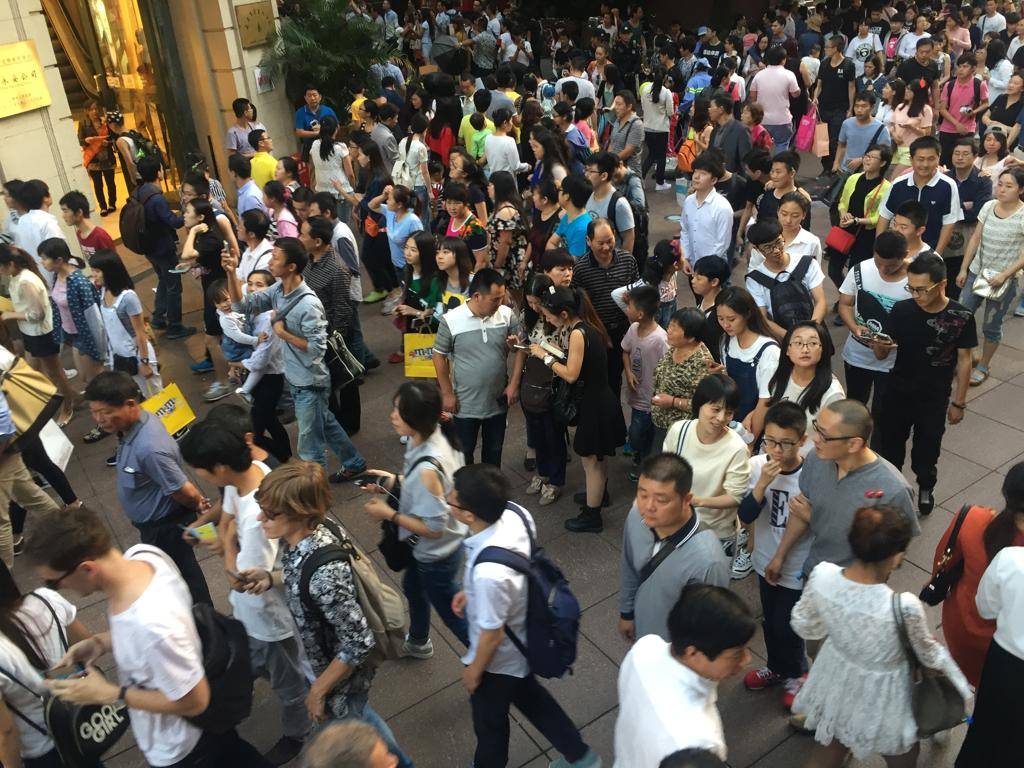
\includegraphics[width=\linewidth]{experiment/images/IMG_236.jpg}
        \end{subfigure}
        \hfill
        \begin{subfigure}{0.3\textwidth}
            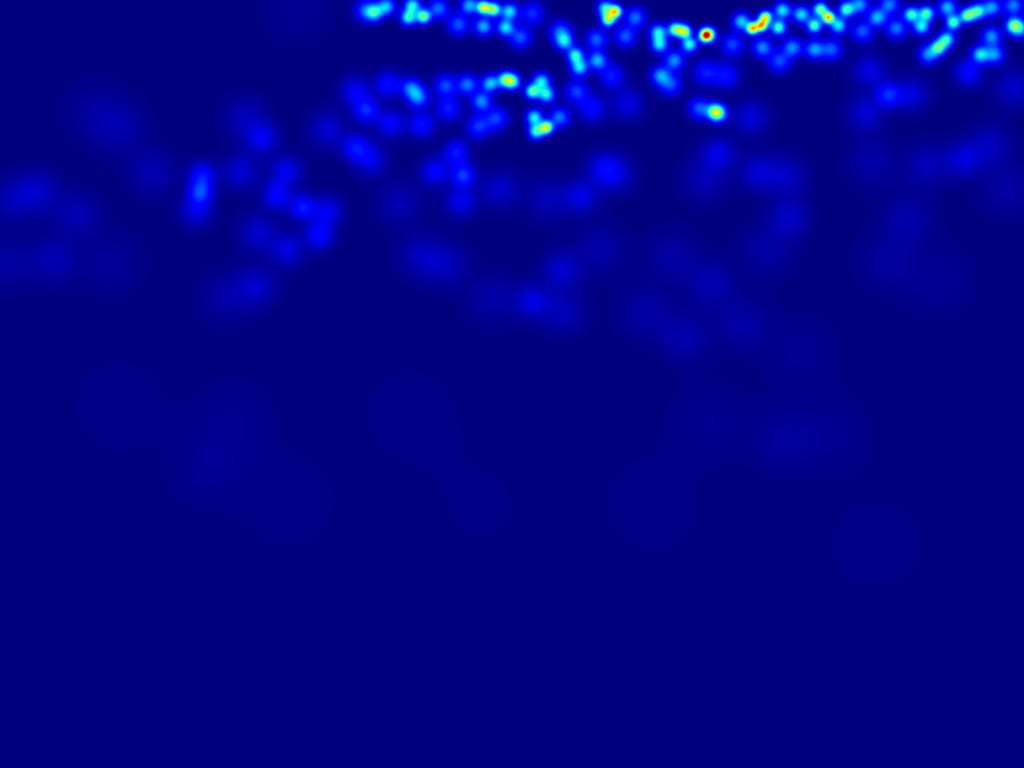
\includegraphics[width=\linewidth]{experiment/images/gt_236.png}
        \end{subfigure}
        \hfill
        \begin{subfigure}{0.3\textwidth}
            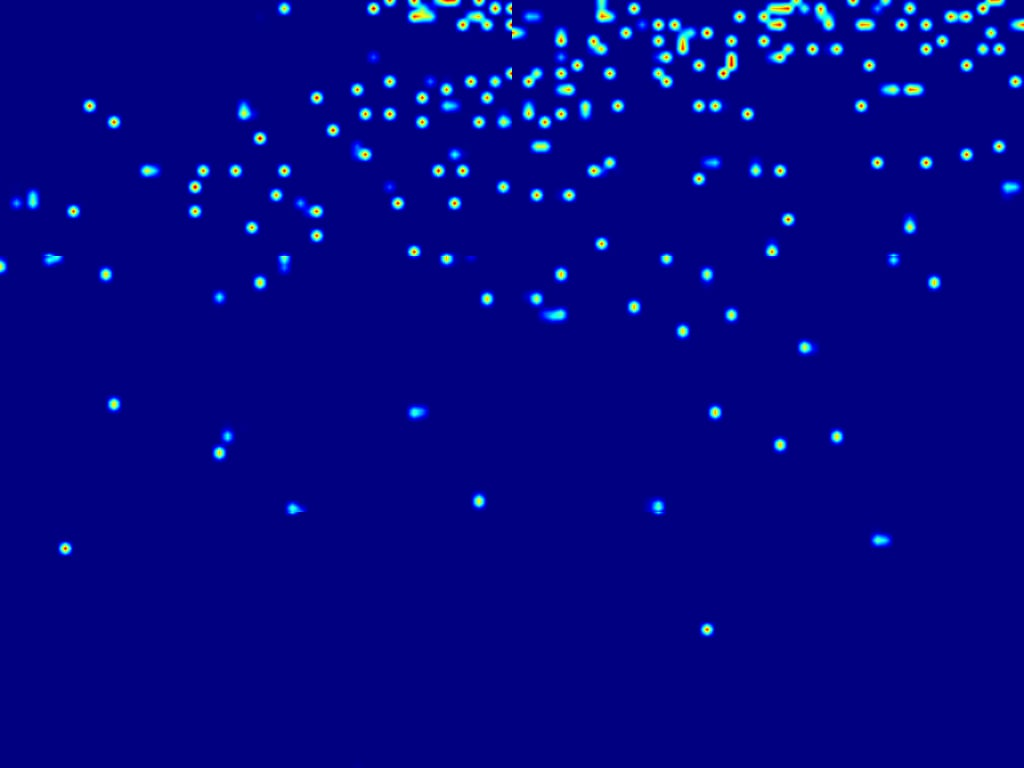
\includegraphics[width=\linewidth]{experiment/images/pred_236.png}
        \end{subfigure}
        \vspace{0.3em}
        \\
    \end{subfigure}

    \vspace{1em} % <--- khoảng cách giữa hai hàng

    % ==== Row 2 ====
    \begin{subfigure}{\textwidth}
        \centering
        \begin{subfigure}{0.3\textwidth}
            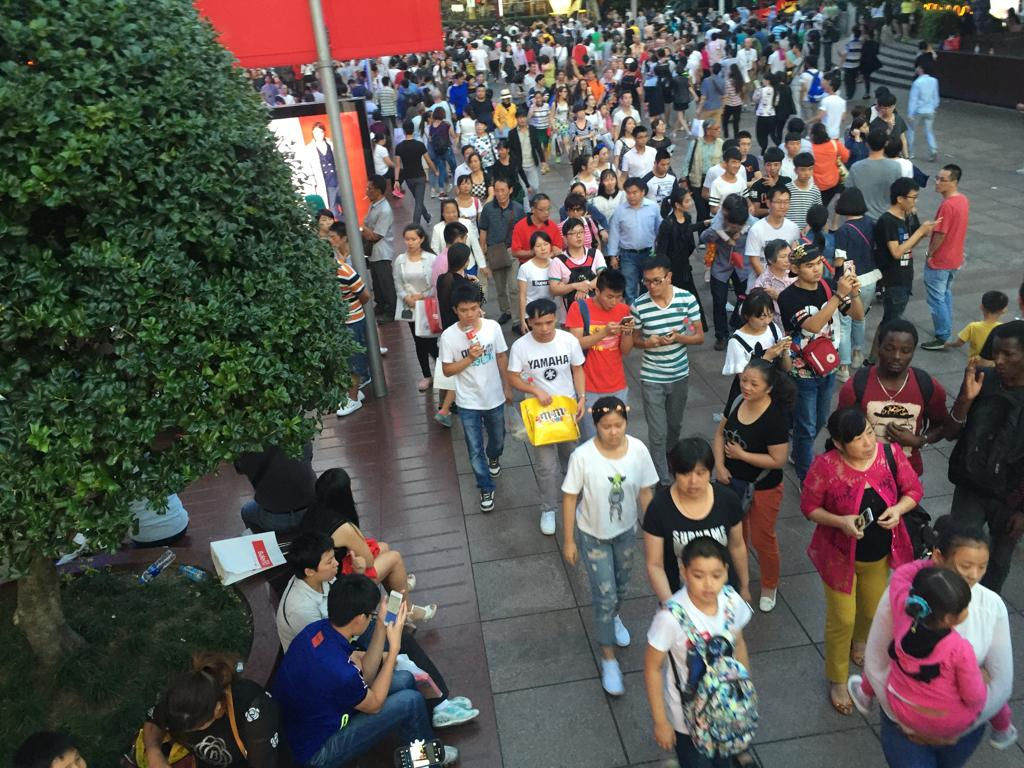
\includegraphics[width=\linewidth]{experiment/images/IMG_237.jpg}
        \end{subfigure}
        \hfill
        \begin{subfigure}{0.3\textwidth}
            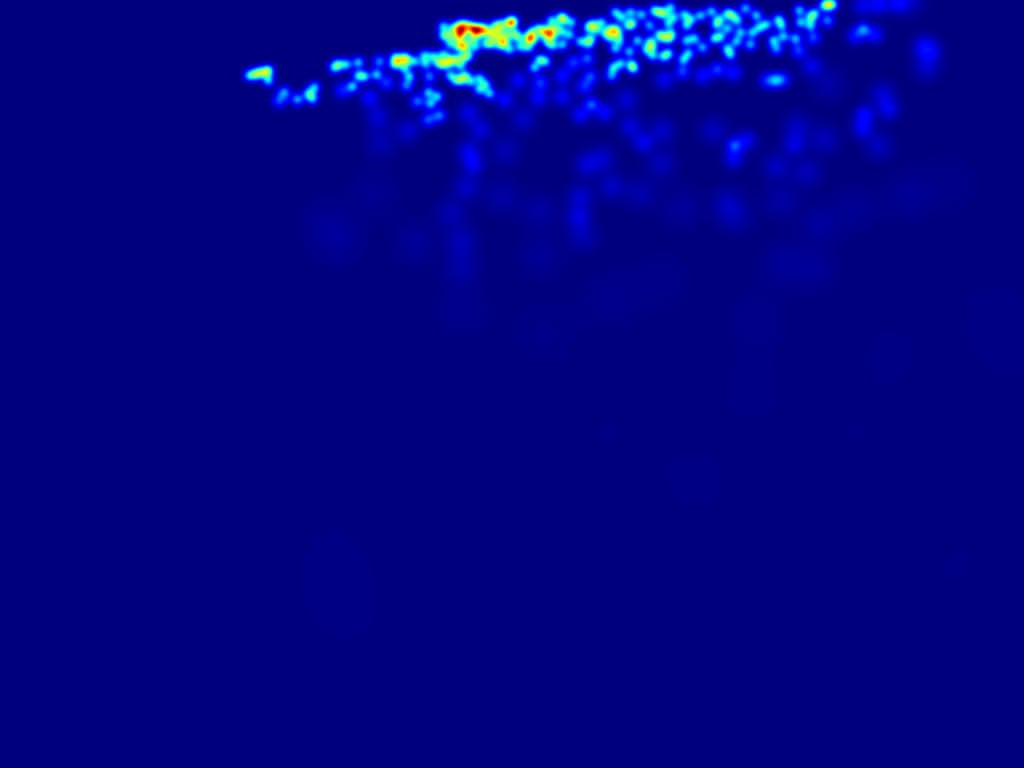
\includegraphics[width=\linewidth]{experiment/images/gt_237.png}
        \end{subfigure}
        \hfill
        \begin{subfigure}{0.3\textwidth}
            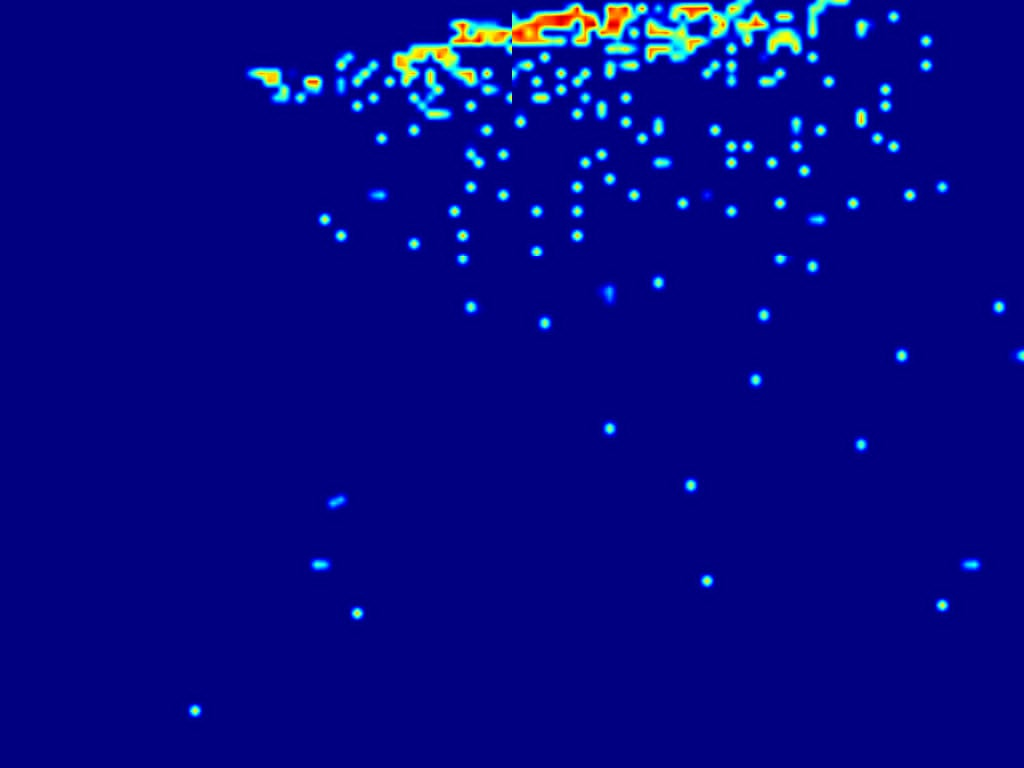
\includegraphics[width=\linewidth]{experiment/images/pred_237.png}
        \end{subfigure}
        \vspace{0.3em}
        \\
        \begin{subfigure}{0.3\textwidth}
            \centering \caption*{Image}
        \end{subfigure}
        \hfill
        \begin{subfigure}{0.3\textwidth}
            \centering \caption*{Ground-truth}
        \end{subfigure}
        \hfill
        \begin{subfigure}{0.3\textwidth}
            \centering \caption*{Prediction}
        \end{subfigure}
    \end{subfigure}

    \caption{Visualization results of CCTrans on the SHB dataset. Each row contains the input image, the corresponding ground-truth, and the prediction.}
    \label{fig:cctrans_results}
\end{figure}
\subsubsection{Metrics}
To quantitatively evaluate the performance of the crowd counting model, we adopt two widely used error metrics: Mean Absolute Error (MAE) and Mean Squared Error (MSE). These metrics are defined as follows:\\
\textbf{Mean Absolute Error (MAE)} measures the average absolute difference between the predicted count and the ground-truth count:
    \[
    \text{MAE} = \frac{1}{N} \sum_{i=1}^{N} | \hat{y}_i - y_i |
    \]
    where \( \hat{y}_i \) is the predicted count for the \(i\)-th image, \( y_i \) is the corresponding ground-truth count, and \( N \) is the total number of test images.

\textbf{Mean Squared Error (MSE)} measures the average of the squared differences between predicted and actual counts, which penalizes larger errors more heavily:
    \[
    \text{MSE} = \sqrt{ \frac{1}{N} \sum_{i=1}^{N} ( \hat{y}_i - y_i )^2 }
    \]

Lower MAE and MSE values indicate better performance, with MAE focusing on overall accuracy and MSE highlighting the presence of outliers. These metrics provide a reliable way to assess the effectiveness of the model in estimating crowd sizes.
\subsection{Comparision between models}
\subsubsection{Counting performance}
CNN-based methods continue to dominate the field of crowd counting, with most models leveraging convolutional neural networks as their core architecture. As illustrated in \ref{table:counting_metrics}, our approach surpasses these methods, showing clear advantages across multiple benchmark datasets and achieving state-of-the-art (SOTA) or near-SOTA performance. Even when compared with more recent transformer-based models, our method consistently delivers superior results in most evaluation,\\
\begin{table*}[htbp]
\centering
\resizebox{\textwidth}{!}{%
\begin{tabular}{lllcclcccccccc}
\toprule
\textbf{Method} & \textbf{Venue} & \textbf{Backbone} & \textbf{Parameters} & \textbf{FLOPS} & \multicolumn{2}{c}{\textbf{SHB}} \\
\cmidrule(lr){6-7} \cmidrule(lr){8-9} \cmidrule(lr){10-11}
& & & & & MAE & MSE \\
\midrule
Yolov11 nano (finetuned) & - & - & \textbf{2.6M} & \textbf{6.5G} & 27.94 & 55.2 \\
CCTrans (own) & arXiv21 & Twins-SVT & 103.58M & 99.44G  & \underline{9.1} & \underline{14.6} \\
FFNet \cite{gao2025effectiveness} & - & ConvNeXt-T & 
\underline{29.02M} & \underline{23.67G} & \textbf{6.1} & \textbf{9.0} \\
\bottomrule
\end{tabular}%
}
\caption{Compared with the advanced methods on ShanghaiTech B. (The best results are shown in \textbf{bold}, and the second best results are \underline{underlined}.)}
\label{table:counting_metrics}
\end{table*}
\subsubsection{Parameters and Computational Resources}
We measured the lightweight characteristics of the model based on two metrics: model parameters and floating-point operations (FLOPs). Among them, the model parameters is one of the key indicators for measuring the complexity of neural network models. It refers to the total number of weights and bias parameters in the model. Models with fewer parameters occupy less storage resources, have faster inference speeds, are easier to deploy, and have lower risks of overfitting. FLOPS is another important metric for measuring the complexity and computational requirements of neural network models. In the experiment, it refers to the number of floating-point operations required for one forward pass. Models with lower FLOPS consume fewer computational resources, have faster inference speeds, are more suitable for low-power environments, and are easier to deploy on mobile and embedded devices.\\
Based on evaluation metrics including accuracy, number of parameters, and floating-point operations (FLOPs), FFNet is selected as the optimal model. It achieves the highest accuracy while maintaining significantly fewer parameters and lower FLOPs compared to YOLO. This demonstrates that FFNet is not only computationally efficient but also more suitable for deployment on resource-constrained devices such as embedded systems or Jetson platforms. Additionally, its lightweight nature helps reduce the risk of overfitting and improves inference speed.
\subsubsection{FFNet on Deep Stream}
\begin{table}[H]
\centering
\begin{tabular}{@{}lccc@{}}
\toprule
\textbf{Method} & \textbf{MAE} & \textbf{RMSE} \\ \midrule
Using WavemixSR    & 40.962606          & 64.914575          \\ 
Without using WavemixSR    & 39.613343         & 60.562368        \\
\end{tabular}
\caption{Performance metrics comparing our proposed end-to-end pipeline and using raw images.}
\label{tab:deepstream_metrics}
\end{table}
We conducted real-time image streaming and inference using DeepStream on the Jetson Xavier platform. Due to current implementation limitations, the sliding window technique—commonly used during inference in our PyTorch-based experiments—has not yet been incorporated into the DeepStream pipeline. This constraint may negatively impact the overall performance of the model, particularly for high-resolution or densely populated scenes where local context is crucial.\\
For the baseline setup without using WaveMixSR, we resized the input images directly to 512×512 and fed them into the FFNet model for inference. This straightforward resizing approach helps reduce computational load but may lead to loss of detail in dense crowd scenes.\\
In contrast, for the setup with WaveMixSR, we first downscaled the original image to 256×256 and passed it through the WaveMixSR super-resolution model. The output of WaveMixSR—an enhanced 512×512 image—was then streamed to the Jetson Xavier and processed by the FFNet model. This approach aims to recover lost visual information and improve feature representation before crowd estimation.\\
As presented in \ref{tab:deepstream_metrics}, the FFNet model using WaveMixSR achieved a Mean Absolute Error (MAE) of 40.96 and Root Mean Square Error (RMSE) of 64.91, while the version without WaveMixSR achieved a slightly lower MAE of 39.61 and RMSE of 60.56. Although the model without WaveMixSR shows marginally better numerical performance in this case, the integration of WaveMixSR still holds promise, especially in scenarios where the input image quality is poor or when higher visual fidelity is necessary for accurate crowd estimation.\\
Moreover, the use of WaveMixSR can be particularly beneficial for deployment in real-world conditions, such as low-resolution surveillance feeds or mobile camera input, where enhancing image quality prior to inference can lead to more stable and interpretable outputs. Future work could explore combining super-resolution with sliding window inference on DeepStream to further close the performance gap with offline models and maximize deployment efficiency.